\chapter{Shape Detection and Clustering}
\label{chap:shapeDetection}

This chapter gives an overview of the shape detection and processing pipeline and presents a clustering algorithm to create a larger-scale representation of a geometric shape from small individual shapes. 
Shape detection is an automated approach to detect geometric primitives in point clouds. Results are usually computed offline, as the computation takes an extensive amount of time. This thesis utilizes an automated shape detection algorithm by Schnabel et al. \cite{schnabel-2007-efficient} that is capable of detecting different types of primitive shapes. It is designed to find shapes in point clouds that consist of several million points within minutes. However, when looking at the performance for smaller samples, results can be achieved at interactive time rates. 

\par

Shape clustering describes the procedure of creating a larger coherent shape from the detected primitive shapes using a selected shape as an initial start. The focus of clustering is to provide the user with information of larger-scale geometry around the region of a selected base shape. 


\section{Overview}

Section \ref{sec:schnabel} describes the algorithm for shape detection in point clouds in depth. Since some of the detected shapes are of infinite size, they need to be refitted to encapsulate the corresponding support points and create a minimal boundary. Section \ref{sec:Refitting} proposes a postprocessing step to refit a primitive shape onto a point set, such that the size of the shape is kept minimal. 

\par

The goal of this thesis is to perform shape detection semi-automatically. Rather than performing shape detection on the complete point cloud, the procedure is executed only on a small subset of points, namely the content of a single octree node, at a time. Performing shape detection on single nodes of the point cloud results in shapes whose size is limited to the extents of the octree node. However, we assume that shapes are presumably a part of a larger structure. 

The start point for the clustering process is a single user-selected shape, called base shape. From this base shape, the algorithm creates a coherent shape cluster that represents the local geometry on a larger scale. Section \ref{sec:shapeMatching} proposes a set of heuristics to determine if two primitive shapes can be combined, thus creating a larger coherent shape. 
Section \ref{sec:shapeClustering} describes the clustering procedure in detail. The resulting homogeneous shape cluster can later be used for user interactions and rendering. 


\section{Efficient RANSAC for Point-Cloud Shape Detection}

\label{sec:schnabel}

The section gives a brief overview over the algorithm used to detect primitive shapes. 
Schnabel et al. \cite{schnabel-2007-efficient} propose an automated way to detect simple primitive shapes in unstructured point clouds. The point cloud is decomposed into a set of shapes and a set of unused points. The algorithm supports detection of planes, spheres, cylinders, cones, and tori. 

\par

\textbf{RAN}dom \textbf{SA}mpling \textbf{C}onsensus (RANSAC) was first discussed by Fischler and Bolles \cite{fischler1981random} as a paradigm for model fitting for image analysis and automated cartography. However, this approach can be generalized for points of an origin other than images. The shape detection works as follows: A minimal set is drawn randomly from the point data, and a primitive shape is constructed from it. This shape is called candidate shape. Section \ref{sec:minimal_sets} describes the properties of a minimal set to build a primitive shape. The candidate shape is then tested against all remaining points to determine how many of them are well approximated by this shape. This evaluation is described in Section \ref{sec:scorefun}. After a given number of trials, the candidate shape that approximates the most points is chosen, and next RANSAC iteration is repeated with the remaining points. 

Section \ref{sec:performance} gives an insight of the performance of the shape detection. 


\subsection{Minimal sets}
\label{sec:minimal_sets}

A minimal set is a set of points that are chosen randomly from the point cloud. The points are treated as possible points on the surface of a primitive shape. The primitive shape is considered a candidate shape if a set of rules applies. The rules for each type of primitive shape are as follows: 

\begin{itemize}
    \item \textbf{Plane}: The minimal set of a plane consists of three points $p_0, p_1, p_2$ whose normals do not deviate from the plane's normal more than the angle $\alpha$. 
    
    \item \textbf{Sphere}: The minimal set to construct a sphere shape consists of two points $p_0, p_1$ with corresponding normal vectors $n_0, n_1$. The center $c$ of the sphere is defined by the midpoint shortest line segment between the parametric lines $p_0 + tn_0$ and $p_1 + sn_1$. The radius is constructed by averaging the distance of $p_0$ and $p1$ to $c$.

    \item \textbf{Cylinder}:
    In order to create a cylinder, a minimal set of two points  $p_0, p_1$ with corresponding normal vectors $n_0, n_1$ is used. The direction $d$ of the axis is established by $d = n_0 \times n_1$. The origin $c$ of the cylinder is created by projecting the parametric lines $p_0 + tn_0$ and $p_1 + sn_1$ onto the plane $d \cdot x = 0$ and taking their intersection as origin $c$. The radius is the shortest distance between $p_0$ and the axis $c + ud$
    
    \item \textbf{Cone}:
    For simplicity, the minimal set for a cone consists of three points $p_0, p_1, p_2$, rather than two. For each point-normal pair, a plane is created. The intersection of the three planes defines the apex $c$. To describe the direction of the axis, a plane is constructed from the points \{$c +  \frac{p_0 - c}{||p_0 - c||}$, $c +  \frac{p_1 - c}{||p_1 - c||}$, $c +  \frac{p_2 - c}{||p_2 - c||}$\}. The normal of this plane is the direction $d$ of the cone axis. The opening angle is given as $\omega = \frac{\sum_{i}^{max} (p_i - c)\cdot d}{3}$
    
    \item \textbf{Torus}:
    A minimal set of four points with normals is used, one more than theoretically necessary, However, this eases the computation.
    Two possible rotational axis are found by intersecting the four point-normal lines $p_i +  \lambda n_i$\cite{marshall2001robust}. For each axis, a full torus is estimated, and the torus is chosen that causes the smaller error in respect to the four points. The minor radius is found by projecting the points onto a plane that rotates around the axis. A circle is constructed using three points, whose radius is the minor radius of the torus. The major radius is given as the distance from the circle center to the axis. 


If a minimal set does not qualify for a candidate shape, the set is discarded. If a minimal set fulfills the rules, the corresponding primitive shape is constructed and returned to as a candidate shape. From there on, the candidate shape score is evaluated. 

\end{itemize} 

\subsection{Score function}
\label{sec:scorefun}

The score function calculates the support of the candidate shape. The support is determined by the number of points that are approximated by this shape, i.e., the points roughly follow the curvature of the shape. All remaining points in the point cloud are tested against the candidate shape. Again, for each point to be a support point, the following two rules must apply: 

\begin{itemize}
    \item The distance between the point and the shape must be smaller than $\epsilon$.
    \item The normal of the point must not deviate from the normal of the shape more than a given angle $\alpha$.
\end{itemize}

From all points that fulfill the previous two conditions, only the subset of points is considered that creates the largest connected component embedded in the shape's surface. The candidate shape is valid if the number of support points exceeds a threshold $n$. 


\subsection{Performance}
\label{sec:performance}

\begin{table}
    \centering
    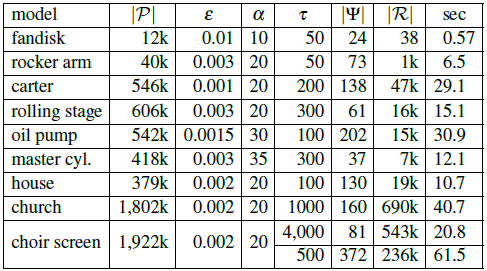
\includegraphics[width=0.7\textwidth]{Shape_Detection/schnabel-performance.png}
    \caption[Original statistics of the shape detection algorithm by Schabel et al.]{The original statistics by Schnabel et al. \cite{schnabel-2007-efficient} on processed models. $\epsilon$ is chosen as a constant fraction of the bounding box width. Results have been averaged over 5 runs and rounded.}
    \label{table:schnabel_performance}
\end{table}

Table \ref{table:schnabel_performance} describes the statistical results for different models. $|P|$ is the number of points, $\epsilon$ the distance threshold, $\alpha$ the maximum normals deviation, $\tau$ is the minimum number of support points, $|\Psi|$ the number of shapes found, $|R|$ the number of RANSAC iterations. It can be seen that for small a small number of points and weaker constraints the algorithm returns plausible results within a fraction of a second. We utilize this feature the detect shapes in our application for small regions at a time to give immediate feedback to the user. 

\todo{Benchmark on real datasets}


\section{Refitting}
\label{sec:Refitting}

The result of the shape detection algorithm is a set of primitive shapes with their corresponding support points. Planes, cylinder, and cones are returned as infinite shapes. For rendering and interaction, it is necessary to create a finite representation for each shape. The set of support points is used to refit the shape and create a finite representation. Spheres and Tori are finite by definition. Hence, they do not require refitting. 


\subsection{Refitting planes}

Planes are represented by a point and a vector. All support points are projected onto the plane, thus reducing the fitting problem to two dimensions. The procedure starts by computing the convex hull of the projected points with the help of Andrew's monotone chain 2D convex hull algorithm \cite{andrew1979another}. 
For this purpose, a bounding quad is used as the representation of the plane. The quad is obtained by using the minimum-bounding-rectangle algorithm by Freeman \cite{freeman1975determining}. Arikan et al. \cite{arikan-2013-osn} take this plane fitting process a step further. Rather than using a rectangular shape in the reconstruction work, an additional polygonization step is performed that extracts a more complex boundary. However, for this thesis the use of a rectangular quad is sufficient.  


\subsection{Refitting cylinders}

A cylinder is defined by a center $p$, direction vector $v$ and a radius $r$. The height of the cylinder is chosen as the maximum distance between two support points on the axis of the cylinder. This is achieved by projecting all points onto the axis $a = p + vt$ of the cylinder, and selecting the points $p_{min}$, where $t$ is minimum and $p_{max}$, where $t$ is maximum. The distance $d$ between $p_{min}$ and $p_{max}$ is the height of the enclosing cylinder. The cylinder is refitted such that the new center is set to $p' = p_{min}$ and the $d$ is encoded in the length of the new direction vector: $v' = \frac{v}{|v|}d$. The radius stays the same. 


\subsection{Refitting cones}

A cone is defined by its apex $c$, axis direction $v$, and opening angle $\theta$. Similar to the cylinder, all support points are projected onto the axis and the points $p_{min}, p_{max}$, with minimum and maximum $t$, are selected. Since the apex of a cone is fixed, the range cannot be encoded using $c$ and $v$. The range is stored separately. Range checks are performed when rendering or interacting with cones. 


\section{Shape-Detection Parameter Selection}
\label{sec:shapeDetectionParameterSelection}

This section briefly discusses the issue of selecting optimal parameters for the shape detection. The $\epsilon$ parameter creates an $\epsilon$-band that follows the curvature of the shape. All points within this $\epsilon$-band are considered to be candidates. The authors propose to use the largest dimension of the point cloud's bounding box times $0.1$ as $\epsilon$. However, using such a static parameter yields problems with extremely sparse regions and regions that are populated very densely. In this thesis, shape detection is performed semi-automatically on local regions of the point cloud at a time. The density of this region, calculated by averaging the distances of each point to its nearest neighbor, is chosen as $\epsilon$. Thus, regions that are populated more densely create finer geometry. 

The $\alpha$ parameter is used to determine the deviation between two directions. As the normals are the same at different levels of detail, this parameter is static. We use an $\alpha$ value of $0.95$. 

The minimum number of support points $n$ per shape is set to $250$. While performing tests for this thesis, a higher number led increased the number of undetected shapes significantly. Weaker constraints resulted in the detection of falsely-detected shapes. 